\documentclass[conference]{IEEEtran}
\IEEEoverridecommandlockouts
% The preceding line is only needed to identify funding in the first footnote. If that is unneeded, please comment it out.
%Template version as of 6/27/2024

\usepackage{cite}
\usepackage{amsmath,amssymb,amsfonts}
\usepackage{algorithmic}
\usepackage{graphicx}
\usepackage{textcomp}
\usepackage{xcolor}
\usepackage{multirow}
\usepackage{float}
\usepackage{bm}
\usepackage{booktabs}
\usepackage{natbib}

\def\BibTeX{{\rm B\kern-.05em{\sc i\kern-.025em b}\kern-.08em
    T\kern-.1667em\lower.7ex\hbox{E}\kern-.125emX}}
\begin{document}

\title{A Comparative Study of Traditional Models and Deep Learning on Biological Data
}

\author{\IEEEauthorblockN{1\textsuperscript{st} Anqi Chen}
\IEEEauthorblockA{\textit{Z5467296} \\
email address or ORCID}
\and
\IEEEauthorblockN{2\textsuperscript{nd} Haoting Qi}
\IEEEauthorblockA{\textit{Z5532554} \\
email address or ORCID}
\and
\IEEEauthorblockN{3\textsuperscript{rd} Ming Yin}
\IEEEauthorblockA{\textit{Z5548164} \\
tianling9shang@gmail.com}
}

\maketitle

\begin{abstract}
This study compares traditional machine learning models (linear and logistic regression) with deep learning models (MLPs) for predicting abalone age. We evaluated model performance on regression and classification tasks, focusing on predictive accuracy and overfitting. Results indicate that while MLPs outperform traditional models in terms of accuracy, they require extensive hyperparameter tuning and regularization to prevent overfitting. This study highlights the trade-offs between model complexity, accuracy, and interpretability in biological data modeling, aiming to determine whether the added complexity of deep learning provides significant improvements over simpler models.
\end{abstract}

\begin{IEEEkeywords}
Machine Learning, Deep Learning, Linear Regression, Multilayer Perceptron, Overfitting.
\end{IEEEkeywords}

\section{Introduction}

\subsection{Background}

Predicting the age of abalone using physical measurements is a challenging problem in biological data analysis. Traditional methods like linear regression have been widely applied to solve such regression problems due to their simplicity and interpretability. However, these models often struggle to capture complex, nonlinear relationships present in biological data, which limits their predictive power. To address these limitations, more advanced techniques, such as deep learning, have been explored.

The concept of deep learning (DL) was first introduced by Geoffrey
Hinton, known for his work on artificial neural networks which earned him the title as the "Godfather of AI". In 2006, Hinton published a seminal paper in Science \cite{hinton2006reducing}, proposing an unsupervised layer-wise pretraining strategy. This strategy effectively tackled the vanishing gradient problem in training deep neural networks, enabling them to learn hierarchical features more effectively from data. This breakthrough significantly advanced the fields of image recognition, speech processing, and natural language understanding.

Since then, deep learning has seen widespread adoption across academia and industry. Deep neural networks (DNNs) have become fundamental for solving complex tasks, including computer vision, speech recognition, and natural language processing. Deep learning's key strength is its ability to automatically extract complex, nonlinear features from high-dimensional data. Hinton's pretraining method played a crucial role in helping deep networks handle intricate data structures, thereby overcoming the limitations of traditional shallow models.

At the same time, tools like Principal Component Analysis (PCA) and autoencoders have been shown to be effective for feature extraction and dimensionality reduction (Bishop and Nasrabadi, 2006) \cite{bishop2006pattern}. This inspired our approach to feature selection, aiming to balance model complexity and interpretability.


In this paper, we explore the similarities and differences between deep learning
and traditional neural networks, with a focus on their performance in
regression and classification tasks. Using the Abalone dataset, we compare the predictive power of
traditional models such as\textbf{ }linear
regression\textbf{ }and\textbf{ }logistic regression\textbf{ }with deep learning models, and examine the potential of
deep learning to improve prediction accuracy.

\subsection{motivation}

Despite significant advancements in machine learning, there is still a lack of sufficient research comparing the performance of traditional and deep learning models on specific datasets, particularly in biological applications like age prediction from physical measurements. Traditional models, such as linear and logistic regression, are popular due to their simplicity and interpretability, but they struggle to handle complex, nonlinear relationships in data, limiting their predictive capabilities. On the other hand, deep learning models, especially deep neural networks, excel at capturing such relationships, but their performance benefits over simpler models for age prediction using the Abalone dataset remain underexplored.

This project aims to fill this gap by systematically comparing the predictive performance of traditional and deep learning models. By evaluating how well these models handle regression and classification tasks using the same dataset, we seek to determine whether the increased complexity of deep learning leads to significant improvements in predictive accuracy compared to simpler, well-established models.

\subsection{contribution}

In this project, we investigate the predictive performance of traditional machine learning models and deep learning models on the Abalone dataset for age prediction (measured by the number of rings). Specifically, we compare the effectiveness of linear regression, logistic regression, and deep learning models in regression and classification tasks. For the classification task, we focus on distinguishing between abalones aged below 7 and those aged 7 or above based on their physical measurements.

We perform feature selection based on the absolute values of the correlation matrix to reduce dimensionality while retaining key features that are most relevant for accurate age prediction. This approach is a filter method, similar to the feature ranking discussed by Guyon and Elisseeff \cite{guyon2003introduction}. Filter methods are simple, scalable, and effective for high-dimensional datasets.

Our main goals are:
\begin{itemize}
\item To evaluate the performance of linear and logistic regression with and without normalization in predicting age and classifying age groups.
\item To explore the effectiveness of deep learning models, including neural networks implemented in TensorFlow and PyTorch, trained with SGD using various configurations (e.g., different numbers of hidden layers, neurons, and learning rates).
\item To compare the impact of data preprocessing techniques, such as normalization and feature selection, on model accuracy and performance.
\item To analyze and report key performance metrics, such as RMSE, R-squared, AUC, and accuracy, for both regression and classification tasks across 30 experiments, with results documented and compared.
\end{itemize}

Through this study, we aim to determine whether the complexity of deep learning models significantly enhances predictive accuracy compared to traditional models when applied to biological datasets, such as the Abalone dataset.



\section{Methodology}

\subsection{Data description and pre-processing}

This dataset was used to predict abalone age from physical measurements. It contains 4,177 samples with 9 features, where the age of the abalone (measured by the number of rings) serves as the target variable. The details of the data are shown in Figure 1.


\begin{figure}[H]
    \centering
    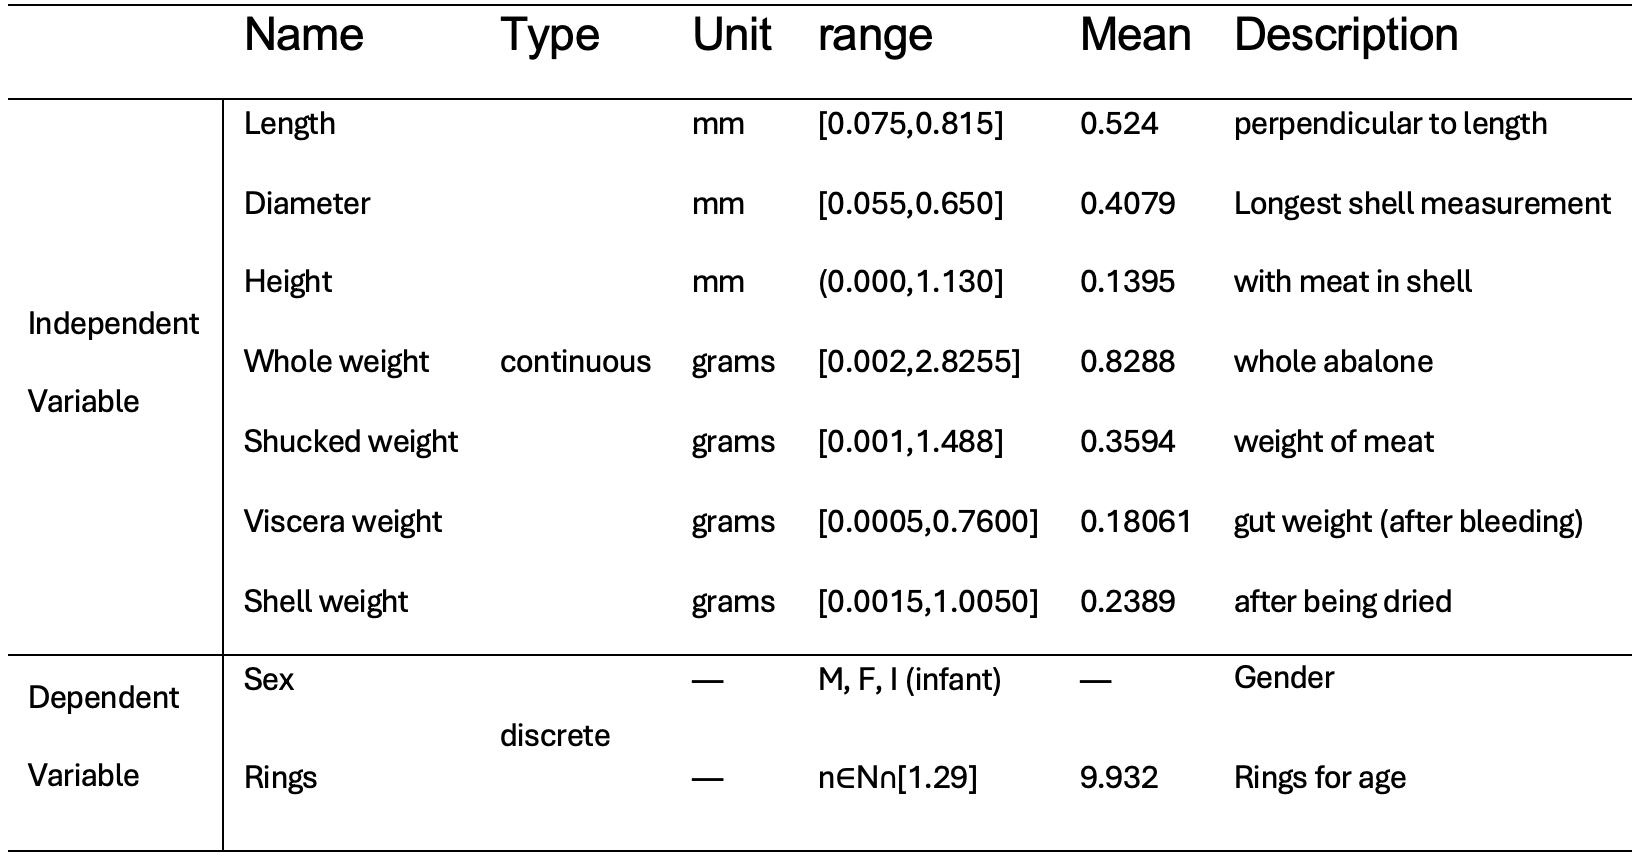
\includegraphics[width=0.5\textwidth]{data_analysis1} % 替换为你的图片文件名
    \caption{Interpretation and distribution of raw data variables}
    \label{fig:example1_image}
\end{figure}

Figure 1 shows that this data is numerical except for the variable Sex, so in this paper, gender M (male) is mapped to 0, F (female) to 1, and I (infant) to 2. as their labels in the model. In order to explore the correlation relationship between the variables, a heat map was used to plot the correlation Figure 2.

\begin{figure}[H]
    \centering
    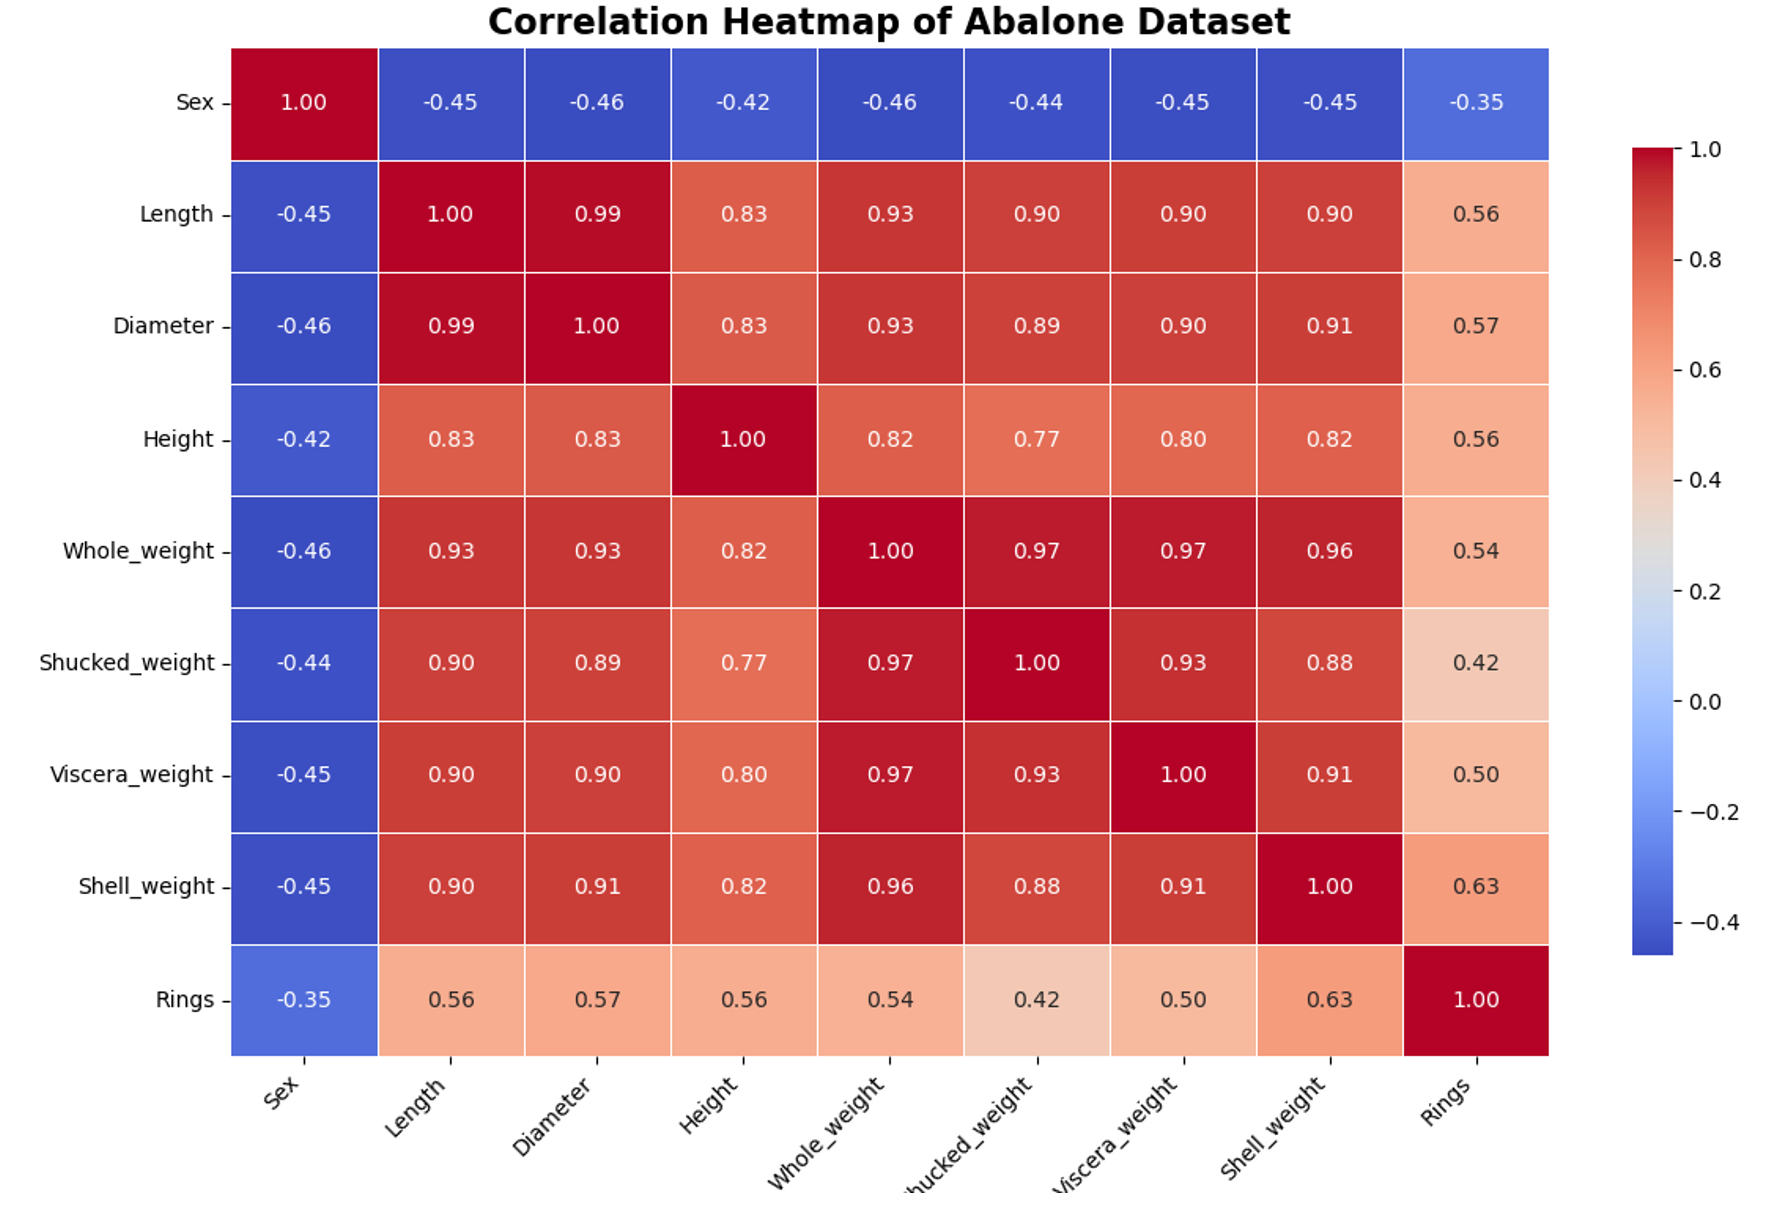
\includegraphics[width=0.5\textwidth]{heatmap} % 替换为你的图片文件名
    \caption{Heat map of correlation between variables}
    \label{fig:example2_image}
\end{figure}

From Figure 2, the correlation between Rings and Shell weight is 0.63, which is the highest correlation of Rings, indicating that shell weight is a better predictor of age. The correlations between Rings and Length, Diameter and Height are between 0.56 and 0.57, indicating that the size of abalone is moderately correlated with age, the larger the size, the older the age may be, but it is not a very strong linear relationship.The correlation between Rings and Sex is -0.35, and there is a weak negative correlation between them.
Using Figure 1, pick the two most relevant variables (one positive and one negative) to Rings, Shell weight and Sex, and create a scatter plot of them against Rings. Due to the large number of samples, there is an overlap of points. The number is indicated by the colour, when the colour is dark there is a high number and when the colour is light there is a low number.

\begin{figure}[H]
    \centering
    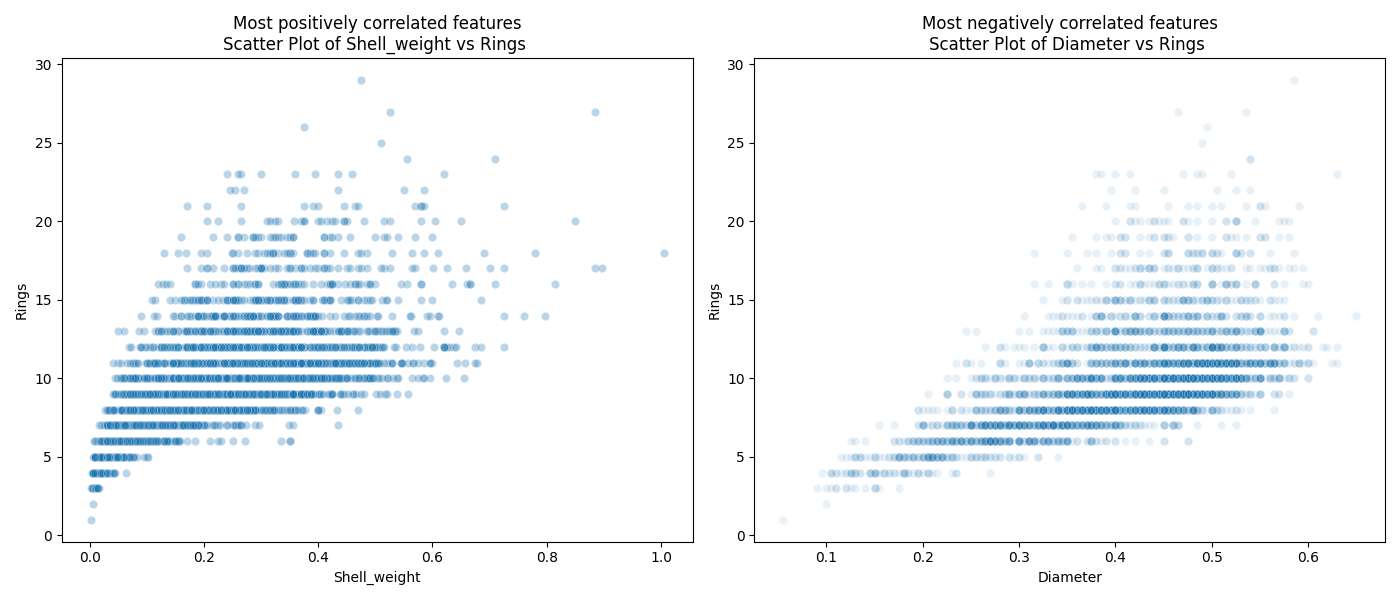
\includegraphics[width=0.5\textwidth]{scatter.png} % 替换为你的图片文件名
    \caption{Scatter plot of Rings versus Shell weight and Diameter}
    \label{fig:example2_image}
\end{figure}

The relationship between Rings and the other two variables can be determined by the colour shades. The first plot in Figure 2 shows that as Shell weight increases, the Rings also tends to increase, and although there is some dispersion in the data, the overall trend is clear. For the second plot, the Rings also increase as diameter increases, but it looks like the increase trend is different from that of shell weight.

\begin{figure}[H]
    \centering
    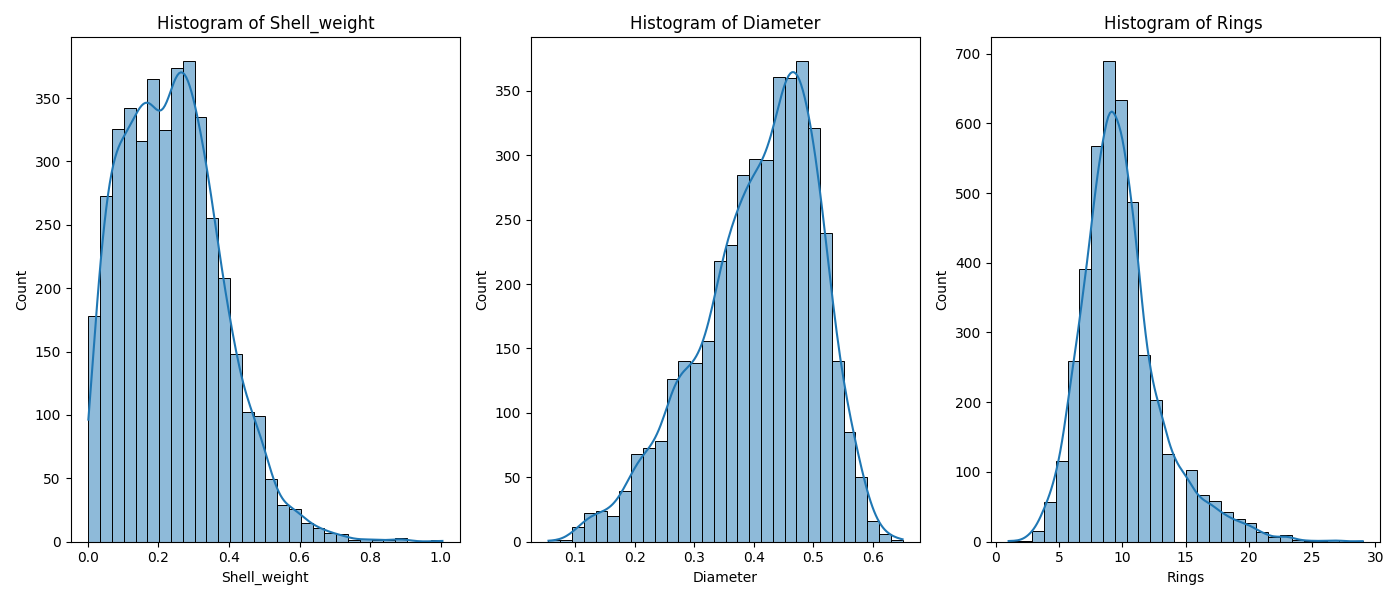
\includegraphics[width=0.5\textwidth]{hist.png} % 替换为你的图片文件名
    \caption{Histograms of Whole weight, Diameter and Rings}
    \label{fig:example2_image}
\end{figure}

For the first graph, the distribution of Shell weight, it can be seen that the distribution of this data shows a clear positive right-skewed, with the majority of shell weights concentrated in the range of 0.1 to 0.4, and a small number of individuals with shell weights above 0.6. Therefore, the values of shell weight are small and concentrated in the low range, with fewer larger shell weights.For the distribution of Diameter, the distribution of the diameter data is close to normal, with most individuals having diameters in the range of 0.3 to 0.5. This indicates that the data are roughly symmetrical.Regarding the distribution of Rings, the image shows a clear positive skewed distribution, with the majority of individuals having a Rings number between 5 and 15, and fewer individuals having a Rings number greater than 20. This indicates that the majority of individuals are young or middle-aged, with only a small number of individuals being older.

\subsection{Model methods}

In this paper, two types of models are used: a linear regression model and a neural network model. The advantages and disadvantages of these models are evaluated by comparing their predictive performance, robustness, and computational cost. The principles of the models are described as follows.

\subsection{Liner model}
Linear models are a class of models for regression and classification tasks that assume a linear relationship between output and input features. In simple linear regression, this relationship is represented by a linear equation. Its mathematical expression is as follows:

\begin{equation}
    y = \beta_0 + \beta_1 x_1 + \beta_2 x_2 + \cdots + \beta_n x_n + \epsilon
\end{equation}

A simplified representation in matrix form is:
\begin{equation}
    y = \mathbf{X} \boldsymbol{\beta} + \epsilon
\end{equation}

In linear regression, for parameter estimation, the most commonly used method for estimating parameters is Sum of Squared Errors (SSE), which finds the best-fitting parameter values by least squares:

\begin{equation}
    SSE = \sum_{i=1}^{n} (y_i - \hat{y}_i)^2 = \sum_{i=1}^{n} (y_i - \mathbf{x}_i \boldsymbol{\beta})^2
\end{equation}

By taking the partial derivatives of the above objective function with respect to \( \beta \) and setting them to zero, a closed solution minimising the sum of squares of the errors can be obtained, which is actually a process of finding the gradient:

\begin{equation}
    \frac{\partial}{\partial \boldsymbol{\beta}} \left[ ( \mathbf{y} - \mathbf{X} \boldsymbol{\beta} )^T ( \mathbf{y} - \mathbf{X} \boldsymbol{\beta} ) \right] = 0
\end{equation}

\begin{equation}
    \hat{\boldsymbol{\beta}} = (\mathbf{X}^T \mathbf{X})^{-1} \mathbf{X}^T \mathbf{y}
\end{equation}

This results in an optimal solution to the linear regression, i.e., the solution that minimises the sum of squared errors. However, the matrix is invertible. When there is multicollinearity between the features,   may not be invertible and regularised regression is required.

\subsection{Logistics model}

Logistic regression is actually a classification algorithm for solving binary classification problems, which predicts the probability of a category and maps the output values of a linear combination via the Logistic function to the [0,1]. The sigmoid function is as follows:

\begin{equation}
    \sigma(\mathbf{X} \boldsymbol{\beta}) = \frac{1}{1 + e^{-\mathbf{X} \boldsymbol{\beta}}}
\end{equation}

At this point the probability is calculated and if classified according to the p(0<p<1), there is the following classification:

\begin{equation}
    \hat{y} =
    \begin{cases}
        1 & \text{if } \sigma(\mathbf{X} \boldsymbol{\beta}) > p \\
        0 & \text{if } \sigma(\mathbf{X} \boldsymbol{\beta}) \le p
    \end{cases}
\end{equation}

Logistic regression uses a Log-Likelihood Function to estimate the model parameters
\( \beta \). The log-likelihood function is of the form:

{\small
\begin{align}
    \mathcal{L}(\boldsymbol{\beta}) = \sum_{i=1}^{n} \left[ y_i \log\left( \hat{P}(y_i = 1 \mid \mathbf{X}_i) \right) + (1 - y_i) \log\left( 1 - \hat{P}(y_i = 1 \mid \mathbf{X}_i) \right) \right]
\end{align}
}

The optimal parameters are found by maximising this log-likelihood function \( \beta \).

\subsection{Neural network}

For the Multilayer Perceptron (MLP) model, which solves regression problems, it is essentially a feed-forward neural network that is trained by a back-propagation algorithm, and SGD is commonly used to optimise the weights. Although MLP is essentially a non-linear model, MLP can be used as a linear regression model if no activation function is introduced.
MLP is consisting of an input layer, a hidden layer and an output layer. Assuming that the model has L layers of neural networks, the output of layer l can be expressed as:

\begin{equation}
    \mathbf{z}^{(l)} = \mathbf{W}^{(l)} \mathbf{a}^{(l-1)} + \mathbf{b}^{(l)}
\end{equation}

Among them: $\mathbf{z}^{(l)}$ is the input of layer $l$ (linear combination), $\mathbf{W}^{(l)}$ is the weight matrix of layer $l$, $\mathbf{a}^{(l-1)}$ is the output of the previous layer, and $\mathbf{b}^{(l)}$ is the bias vector of layer $l$.

For the regression problem, the MLP uses the Mean Squared Error (MSE) as a loss function of the form:

\begin{equation}
    L = MSE = \frac{1}{n} \sum_{i=1}^{n} (y_i - \hat{y}_i)^2
\end{equation}

Next, Stochastic Gradient Descent (SGD) is used to optimise the model parameters. At each iteration, the weights and biases are updated using a small batch or a sample of the dataset, gradually reducing the loss function values. The formula for updating the parameters each time is:

\begin{equation}
    \mathbf{W} = \mathbf{W} - \eta \frac{\partial L}{\partial \mathbf{W}}
\end{equation}

\begin{equation}
    b = b - \eta \frac{\partial L}{\partial b}
\end{equation}

Through continuous iteration, SGD adjusts the weights W and bias b until the loss function is minimised and the optimal linear mapping relation is found.

\subsection{Software suite}

For this experiment, this article mainly who used these libraries in python, its main functions are as follows. We used $Scikit-learn's$\cite{pedregosa2011scikit} $cross-validation$ and grid search tools for model selection and parameter tuning. These tools allowed us to effectively evaluate model performance and select the optimal parameter configuration, thereby improving prediction accuracy.

\begin{figure}[H]
    \centering
    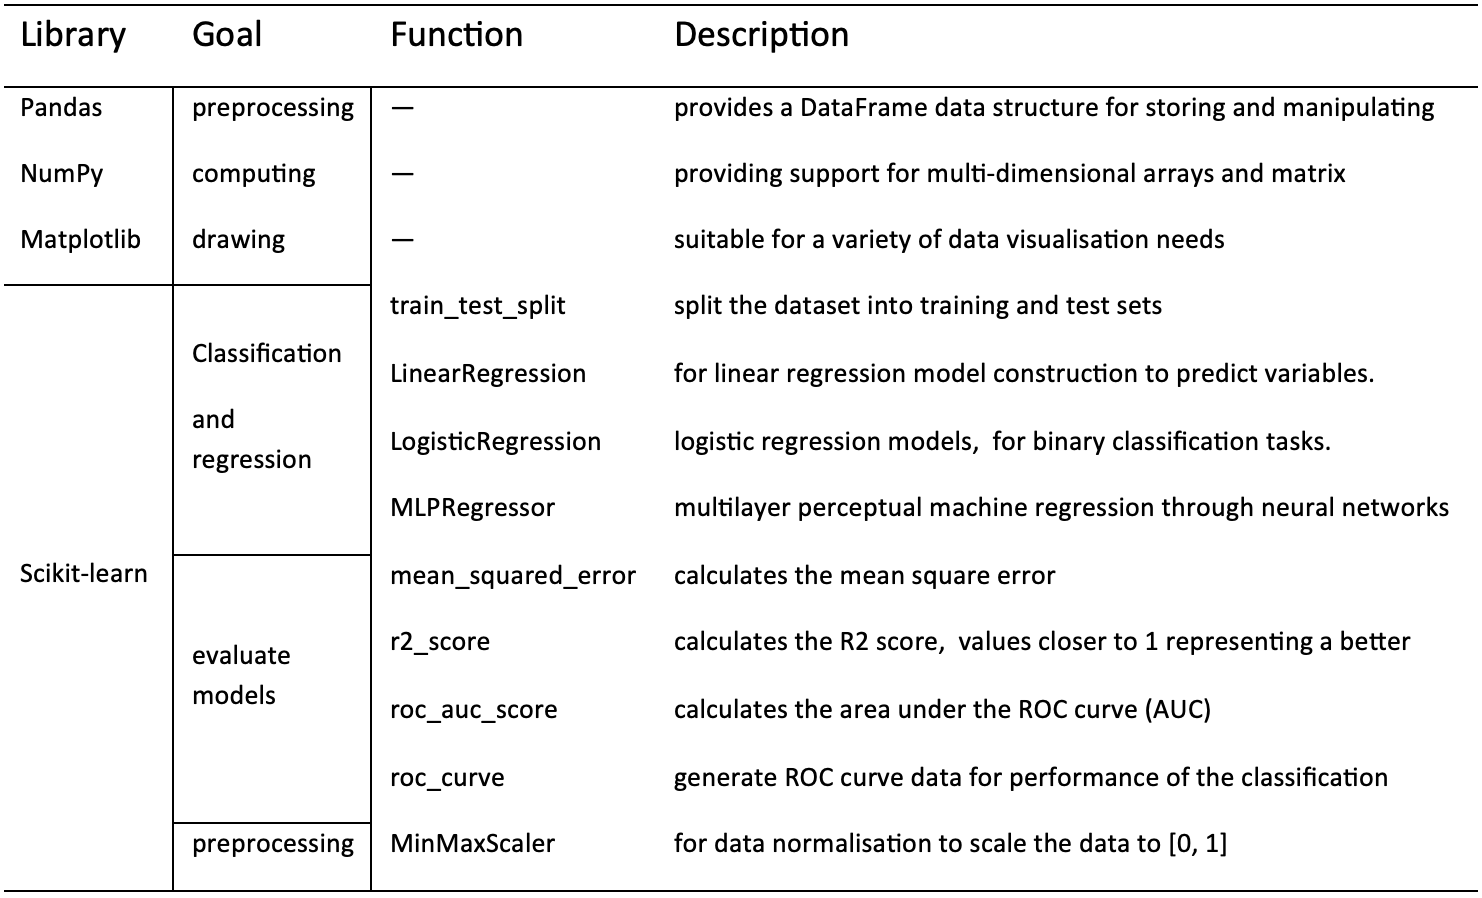
\includegraphics[width=0.5\textwidth]{library.png} % 替换为你的图片文件名
    \caption{Functions used in python and their libraries}
    \label{fig:example2_image}
\end{figure}

In addition to this, this paper sets the random seed through the random.seed function of the random library, and the value of the random seed is related to the number of runs. Thus, the repeatability of the results of this experiment is achieved.


\section{Results}
\subsection{Liner regression}

A linear regression model is constructed to compare the difference between using data that is normalised and using normalised data, and to compare the difference between using all the variables and using only the two most relevant variables. In addition, in order to reduce the disturbance caused by randomness, to a more reliable estimate of the model performance. The experiment was run 30 times and the mean and variance of RMSE and R2 were calculated for a more reasonable assessment of the model fit. The results are shown in Table 1.

\begin{table}[htbp]
    \centering
    \caption{Different types of linear models RMSE and R2}
    \begin{tabular}{|l|l|c|c|c|c|}
        \hline
        \textbf{Value} & \textbf{Data set} & \textbf{all unnorm} & \textbf{all norm} & \textbf{2\_feat\_unn} & \textbf{2\_feat\_norm} \\ \hline
        mean\_rmse & train & 2.183512 & 2.183512 & 2.502071 & 2.502071 \\ \hline
        std\_rmse & train & 0.032705 & 0.032705 & 0.039948 & 0.039948 \\ \hline
        mean\_rmse & test & 2.234785 & 2.234785 & 2.5213 & 2.5213 \\ \hline
        std\_rmse & test & 0.051467 & 0.051467 & 0.060533 & 0.060533 \\ \hline
        mean\_r2 & train & 0.539888 & 0.539888 & 0.395903 & 0.395903 \\ \hline
        std\_r2 & train & 0.011478 & 0.011478 & 0.012943 & 0.012943 \\ \hline
        mean\_r2 & test & 0.520481 & 0.520481 & 0.390007 & 0.390007 \\ \hline
        std\_r2 & test & 0.022482 & 0.022482 & 0.019387 & 0.0193875 \\ \hline
    \end{tabular}
    \label{tab:linear_models_rmse_r2}
\end{table}

For $all\_unnorm$ and $all\_unnorm$ (models using all features, unnormalised and normalised). The RMSE and R² for the training and test sets are almost the same, 2.18 and 2.23 (RMSE) and 0.54 and 0.52 (R²), respectively. The two models are equally effective in explaining the variance of the training and test sets, while their results on normalisation or not are not very different, indicating that normalisation has little effect on the results.
While $2\_feat\_unn$ and $2\_feat\_unn$ (using the two most relevant features, unnormalised and normalised): the RMSE is higher for the training set and the test set, 2.50 and 2.52 respectively, and the R² is lower, about 0.39. This indicates that the model performs poorly and the error increases when only two features are used.
So $all\_unnorm$ and $all\_unnorm$ are the best choice because they have the lowest RMSE and highest R².
The reason why normalisation does not have much effect on the corresponding model for this data is probably because normalisation does not have much effect on linear regression, which is not sensitive to the scaling of the features, and there is not much difference in the scale of the features. Since the RMSE is calculated based on the original value of the target variable y, not on the normalised feature X, the RMSE before and after normalisation usually does not change much, or may not even change at all.

\subsection{Logistic regression}

For logistic regression analysis, evaluating four different scenarios: comparing all features with selected features and the effect of normalization and unnormalization is examined, helps to provide insights into the negative impact of redundant features on the decision-making process of the model. This approach also evaluates the effectiveness of normalization in enhancing model stability and robustness, which helps to improve prediction accuracy and generalization performance to new data. We analyzed two key performance parameters: the AUC Score and the ROC curve. Results indicated that feature selection and normalization positively impact model performance.

\subsubsection{AUC Score}

Table 2 shows the AUC scores for the four scenarios:

\begin{table}[htbp]
    \centering
    \caption{Logistic AUC Analysis}
    \begin{tabular}{lcccc}
        \toprule
        \textbf{feature type} & \textbf{norm flag} & \textbf{min} & \textbf{mean} \\ \midrule
        all & 0 & 0.9266 & 0.9359 \\
        all & 1 & 0.9268 & 0.9360 \\
        selected & 0 & 0.9296 & 0.9374 \\
        selected & 1 & 0.9296 & 0.9374 \\
        \bottomrule
    \end{tabular}
    \label{tab:logistic_auc_analysis}
\end{table}

Key Observations:
\begin{itemize}
\item All features vs. selected features: The AUC performance of selected features is slightly higher than that of all features, indicating that reducing redundant features can improve model performance in this dataset and model.
\item Normalized vs. Unnormalized: According to the data, the average AUC is only about 0.0002 different between normalized and un-normalized, indicating that the standardization of features has insignificant effect on the model performance.
\end{itemize}

Figure 6 shows the results of AUC comparison between the four contexts in 30 experiments, as shown below:
\begin{figure}[h]
    \centering
    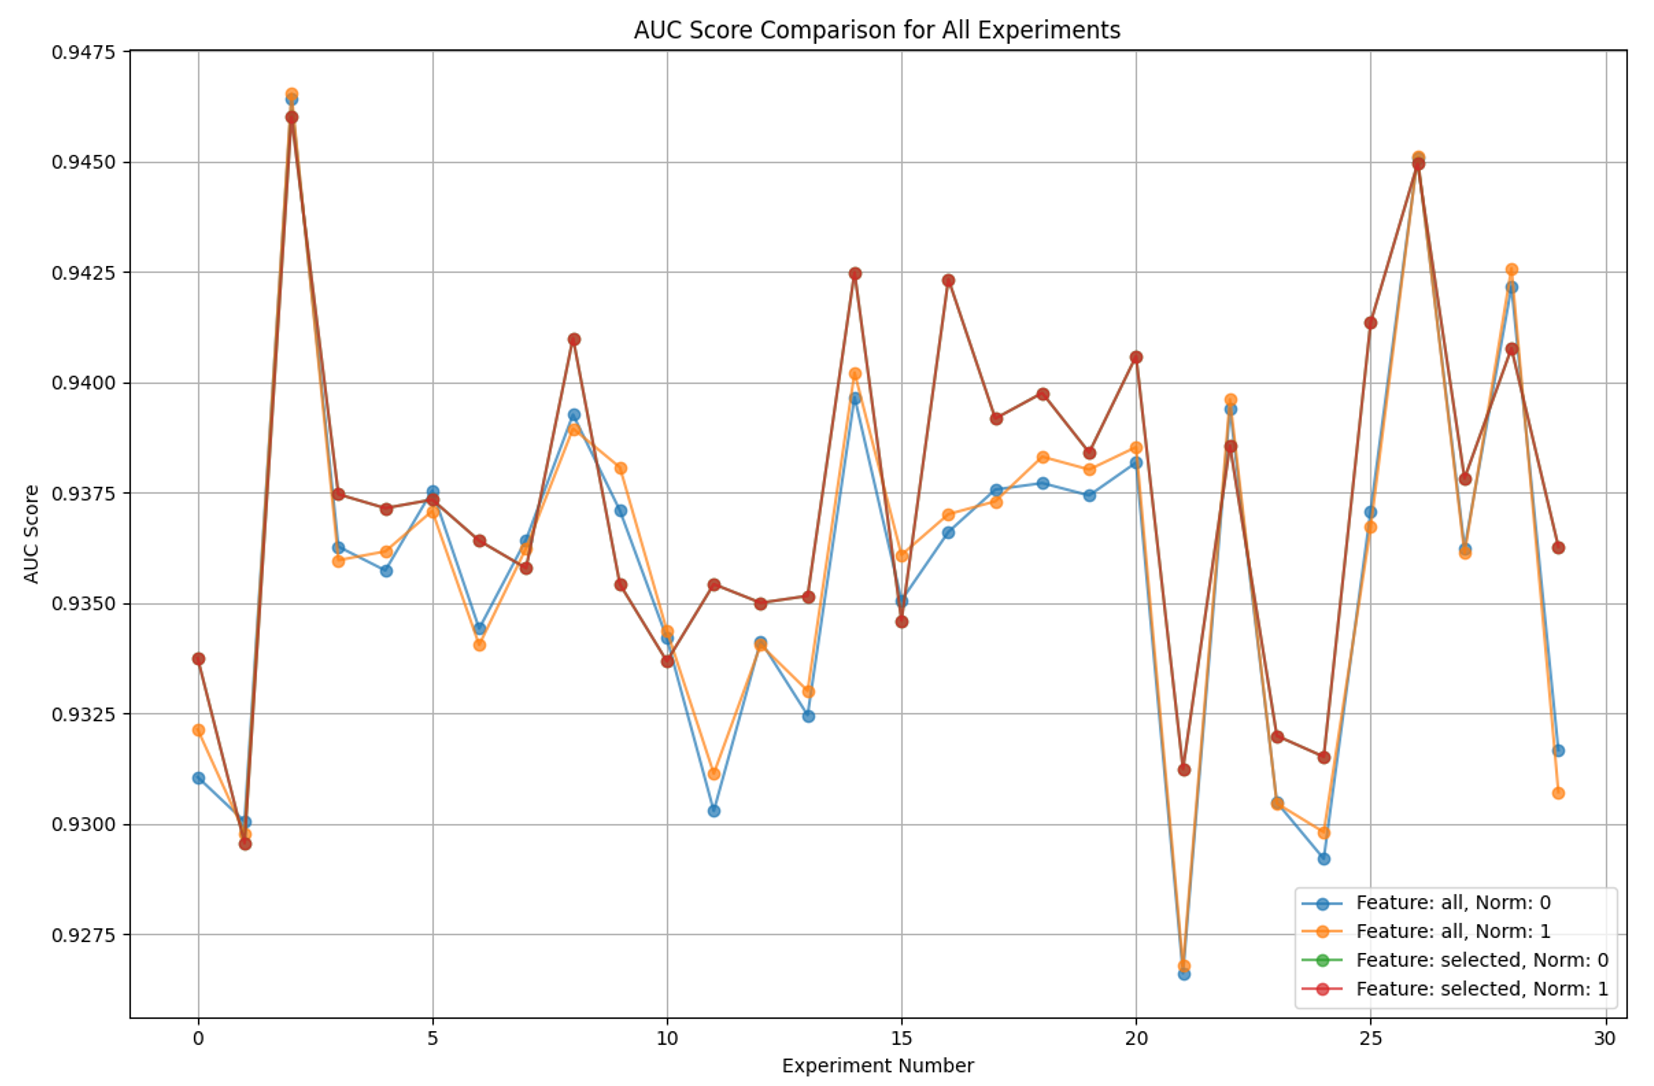
\includegraphics[width=0.5\textwidth]{auc_comp.png} % 替换为你的图片文件名
    \caption{Logistic AUC comparison}
    \label{fig:example1_image}
\end{figure}

Key Observations:
The analysis results show that the AUC score of the feature selected with normalization performs more better. This may be attributed to the fact that feature selection reduces the noise interference on the model decision, while normalization ensures that the features are evaluated on the same scale, which enhances the stability and generalization ability of the model.

\subsubsection{ROC curves }

To further evaluate the reliability of the logistic regression model, we compared the ROC curves from 30 experimental trials. The results indicate that the area under the curve (AUC) remains consistent across trials, which suggests high robustness of the model. Figure 7 shows the ROC curves of two randomly selected experiments for comparison:
\begin{figure*}[h]
    \centering
    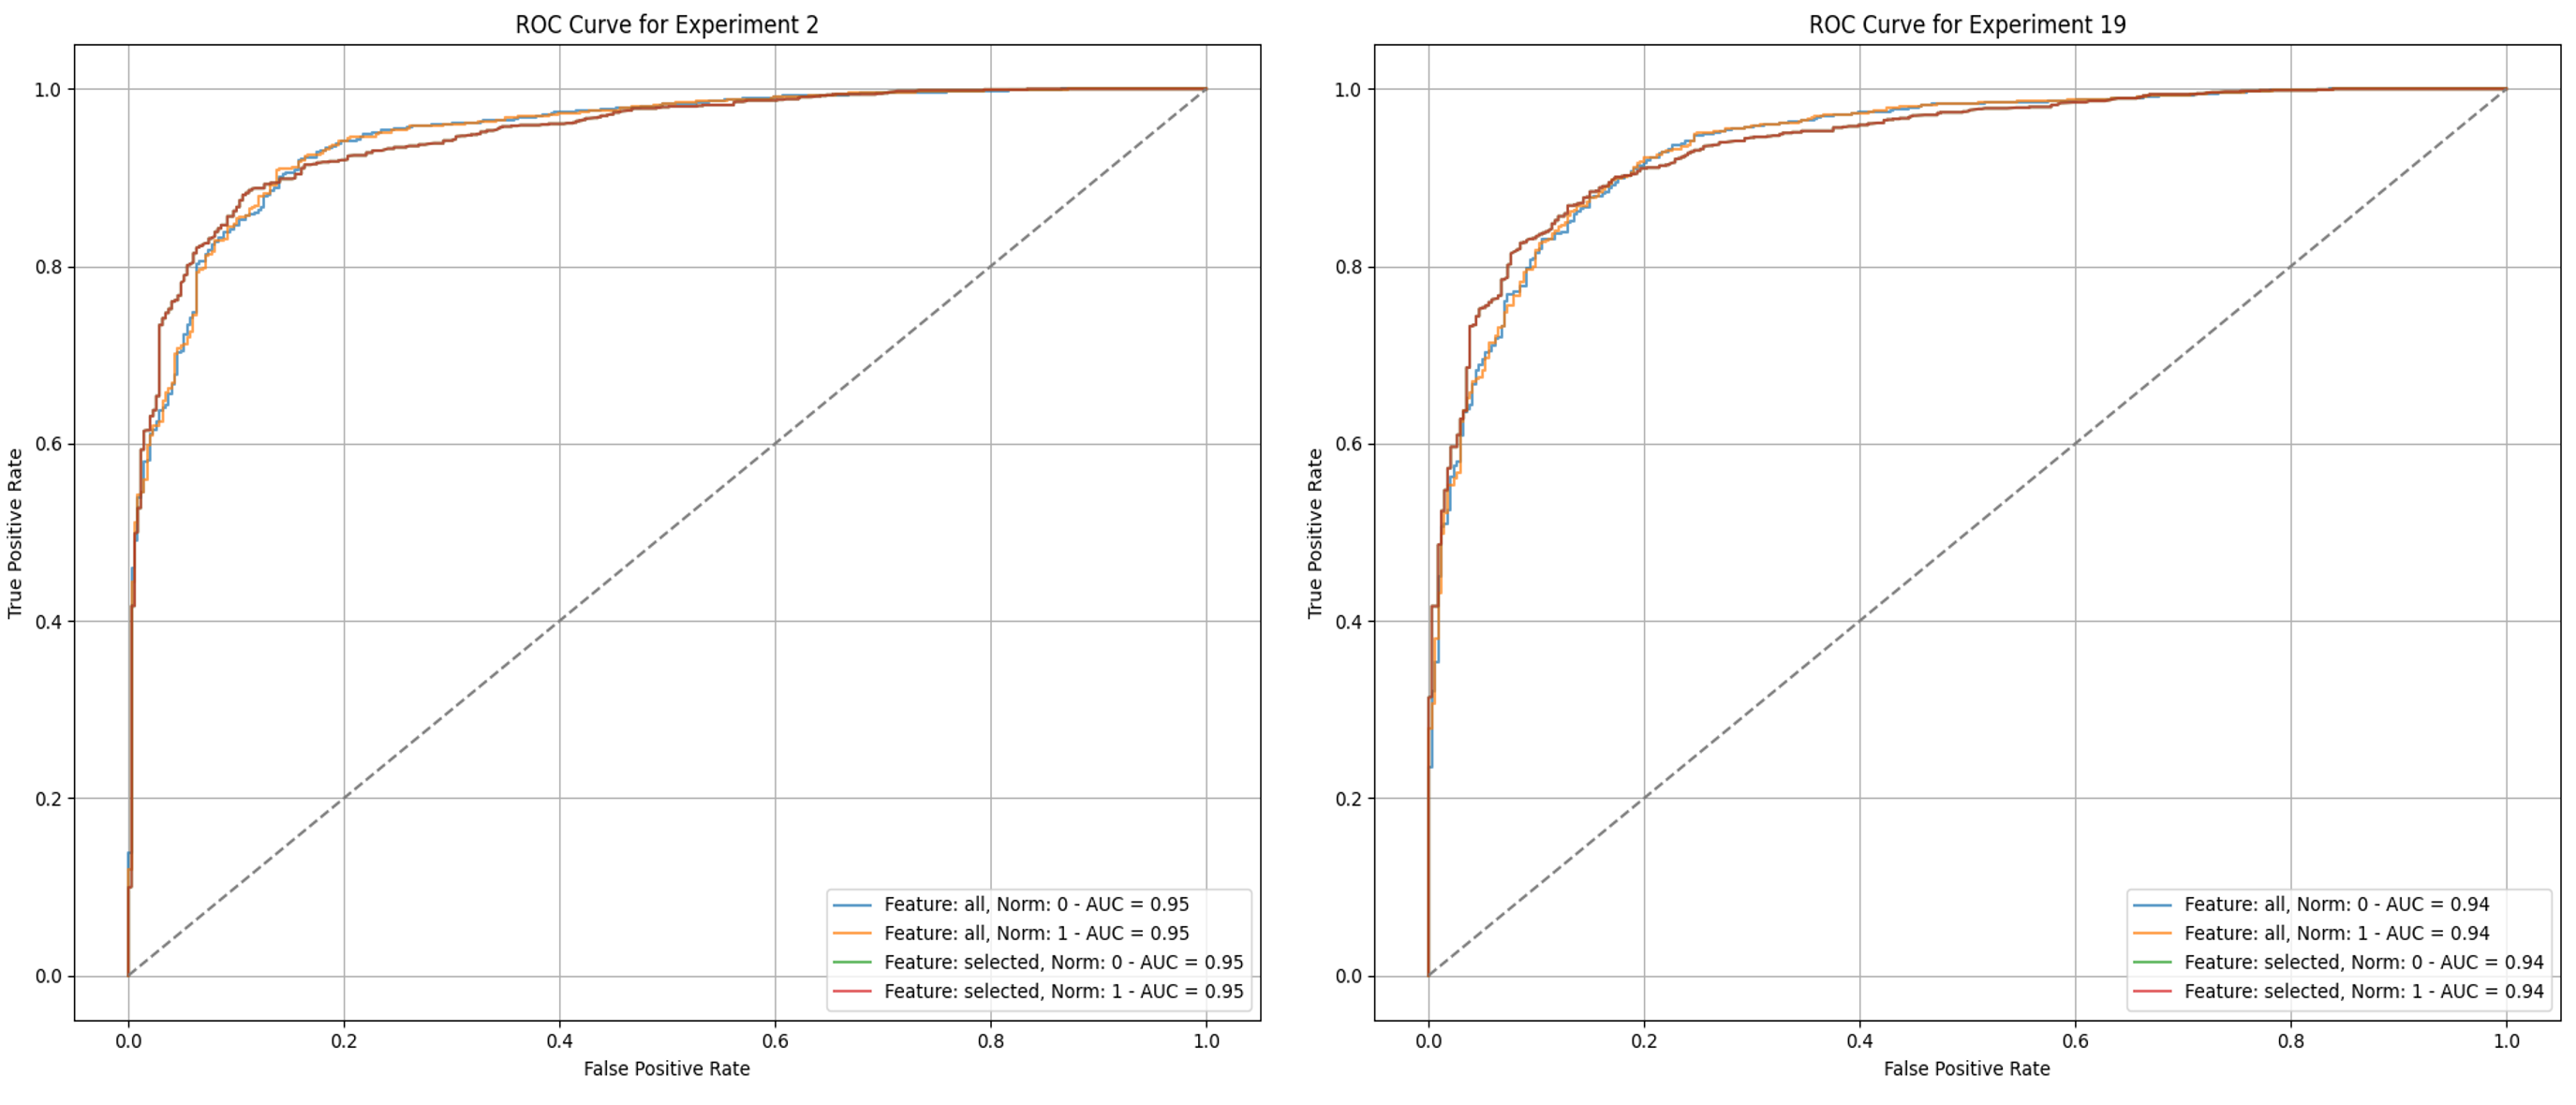
\includegraphics[width=\textwidth]{roc_comp.png} % 替换为你的图片文件名
    \caption{Logistic ROC comparison}
    \label{fig:example1_image}
\end{figure*}

Key Observations:
\begin{itemize}
\item The ROC curves reflect the model’s performance across different thresholds, showcasing its ability to distinguish between positive and negative classes effectively.
\item The consistent AUC values across experiments reinforce the model’s reliability, indicating that the logistic regression model maintains its performance regardless of variations in the training data.
\end{itemize}




\subsection{MLP Neural networks}

This paper attempts to find the neural network construction method that is most suitable for predicting this data. Therefore, three mainstream methods for building multilayer perceptron are used, i.e., using TensorFlow library, Kears library and using Sklearn library respectively. At the same time, in order to maximise the prediction effect of each model, we allow different hyperparameters for each model, i.e., we find the most suitable case for the model by using different permutations of the learning rate, the number of hidden layers and the number of neurons. The optimal hyperparameters found for the different models are given in the table 3.3.1:

\begin{table}[htbp]
    \centering
    \caption{Hyperparameters for different models}
    \begin{tabular}{|l|c|c|c|}
        \hline
        \textbf{hyperparameters} & \textbf{Tronsflow} & \textbf{Kears} & \textbf{Sklearn} \\ \hline
        neurons & 128 & 128 & 10, 5 \\ \hline
        hidden layers & 2 & 1 & 2 \\ \hline
        learning rate & 0.01 & 0.01 & 0.001 \\ \hline
    \end{tabular}
    \label{tab:hyperparameters_models}
\end{table}

Through continuous testing, the most suitable values for the corresponding models were found and the best hyperparameter values were determined for different models.
The different models are run 30 times respectively and the average of the returned RMSE and R2 values are used to determine which training model to use is more suitable for the present model, the results of which are shown in Table 3.2.

\begin{table}[htbp]
    \centering
    \caption{Table 3.3.2 RMSE and R2 of neural networks constructed by different methods}
    \begin{tabular}{llcccccc}
        \toprule
        \textbf{Value} & \textbf{Data set} & \multicolumn{2}{c}{\textbf{Tronsflow}} & \multicolumn{2}{c}{\textbf{Kears}} & \multicolumn{2}{c}{\textbf{Sklearn}} \\ \cmidrule(lr){3-4} \cmidrule(lr){5-6} \cmidrule(lr){7-8}
                       &                   & \textbf{mean} & \textbf{std} & \textbf{mean} & \textbf{std} & \textbf{mean} & \textbf{std} \\ \midrule
        RMSE          & train             & 2.1801 & 0.1225 & 2.2036 & 0.0345 & 2.0783 & 0.0320 \\
                       & test              & 2.2249 & 0.1253 & 2.2282 & 0.0558 & 2.1210 & 0.0493 \\ \midrule
        R2            & train             & 0.5236 & 0.0521 & 0.5314 & 0.0114 & 0.5832 & 0.0100 \\
                       & test              & 0.5408 & 0.0539 & 0.5237 & 0.0132 & 0.5683 & 0.0152 \\
        \bottomrule
    \end{tabular}
    \label{tab:rmse_r2_neural_networks}
\end{table}

For Transflow, the average RMSE of the training set is 2.180 and the average RMSE of the test set is 2.225. The RMSEs of the training and test sets are close to each other, which means that the model is fitted in a stable way and there is no obvious overfitting or underfitting. Meanwhile, the R² of the training set is 0.524, and the R² of the test set is 0.540, the difference between the R² of the training set and the test set is small, which indicates that the model does not have obvious overfitting phenomenon. However, the R² value is slightly lower, indicating that the fit is not optimal.
For Kears, the RMSE of the training set is 2.203 with a standard deviation of 0.034, and the RMSE of the test set is 2.229 with a standard deviation of 0.055. The RMSEs of the training and test sets are very close to each other, and the standard deviation is small, and the model shows high stability. Besides, the R² of the training set is 0.532 and the R² of the test set is 0.524. The R² value is slightly higher than that of Transflow, which indicates that the fitting effect is better, and the R² values of the training and test sets are close to each other, which means that the model is more stable.
In Sklearn, the RMSE is 2.078 for the training set and 2.121 for the test set. it has the smallest RMSE value, which indicates that it has a lower error than the other two models, which suggests that it has the best fit on both the training and test sets. The training set R² is 0.583 and the test set R² is 0.568. it has the highest R² value which indicates that it fits best.

\section{Discussion}
\subsection{Results Summary }

This project evaluates the performance of various methods for age prediction using linear regression, logistic regression models, and neural networks trained with stochastic gradient descent (SGD) on the abalone dataset. The results indicate that the models have achieved our project goals.

The following two figures summarize the evaluation results of the different methods:

\begin{figure}[H]
    \centering
    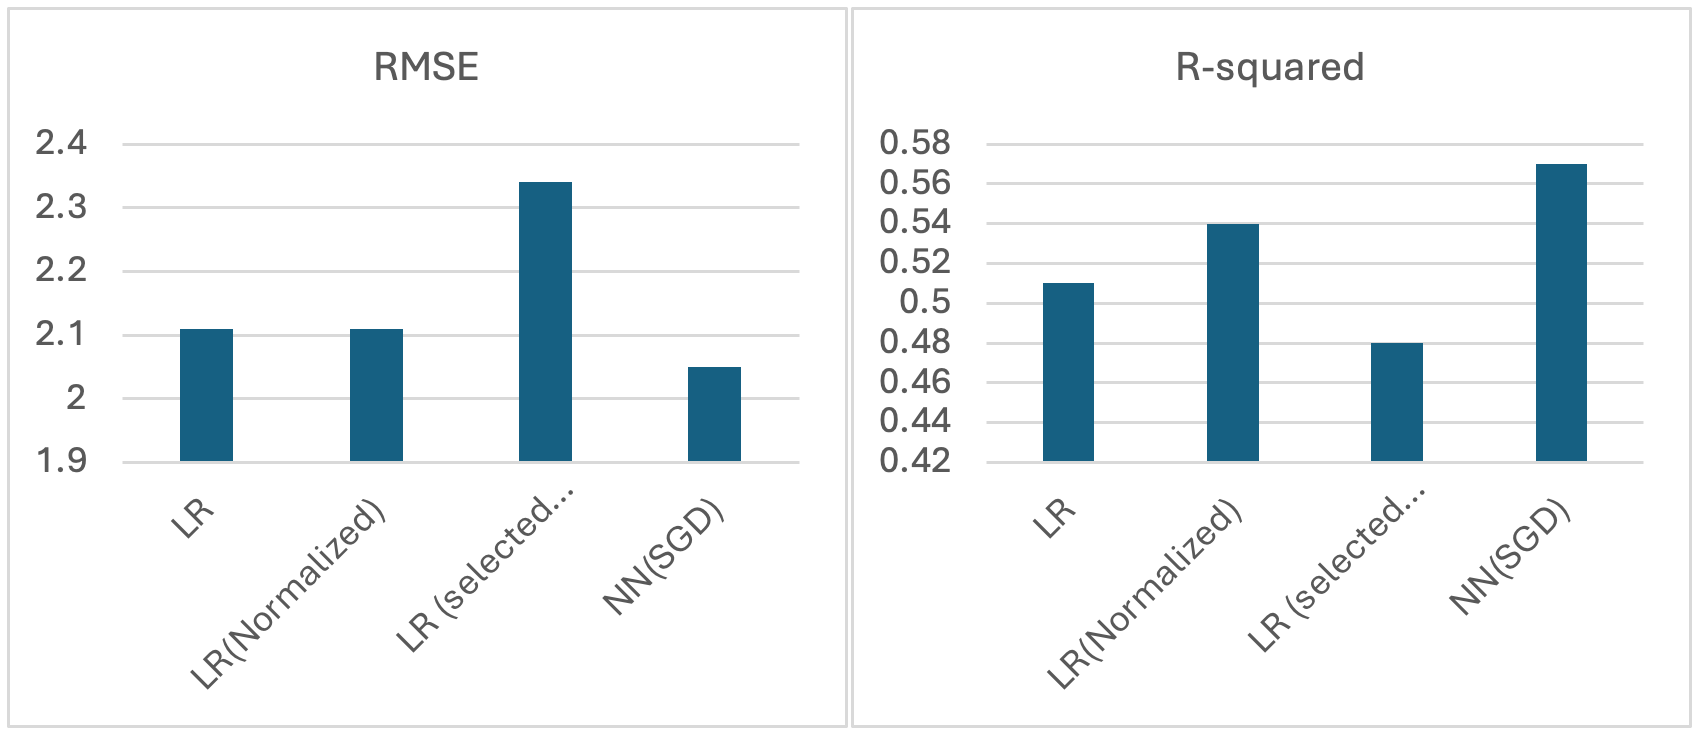
\includegraphics[width=0.5\textwidth]{model_comp1.png} % 替换为你的图片文件名
    \caption{Scatter plot of Rings versus Shell weight and Diameter}
    \label{fig:example2_image}
\end{figure}

Key observations from the data:
The standard linear regression model achieved a root mean square error (RMSE) of 2.11 and an r-squared value of 0.51, indicating moderate predictive ability. Normalizing the features kept the RMSE constant but increased the R-squared to 0.54, indicating that the model fit was enhanced. In contrast, the RMSE of the linear regression model using only two features increased to 2.34, showing a decrease in performance due to the loss of potentially critical information. The neural network model trained using stochastic gradient descent showed a significant advantage with a minimum RMSE of 2.05 and a maximum R-squared of 0.57, highlighting its effectiveness in capturing the complex relationships in the data.

\subsection{Methodology Limitations}
\begin{itemize}
\item Over-fitting

Neural networks typically consist of a large number of parameters, which increases their ability to adapt to complex data models. However, all three training methods showed better performance on the training set compared to the test set, suggesting that over-fitting may be present. Over-fitting occurs when the model captures patterns specific to the training data, resulting in reduced performance on the unseen test data. This suggests that the model may be difficult to effectively generalize to new data, thus affecting its predictive accuracy and robustness in real-world applications.

\item Insufficient Hyper-parameter Search

Despite the initial exploration of neural network models with specific combinations of hyper-parameters (e.g., number of layers, learning rate, etc.). However, the potential capabilities of the models may not have been fully explored due to the more limited scope of configuration search. The restricted space for hyper-parameter tuning may result in the model failing to achieve its theoretically optimal performance, especially when dealing with complex high-dimensional data, making it difficult to fully capture its generalization ability and optimal solution. Further hyper-parameter optimization processes (e.g., grid searches or stochastic searches) are especially necessary to more fully evaluate the model's performance, thus fully exploring the performance limits of neural networks.

\item Insufficient Performance

In this project, the highest R-squared value obtained by the model is about 0.57, indicating that it has significant limitations in explaining the variance of the dependent variable, and that the currently adopted neural network architecture may be too simple to effectively capture the underlying complex relationships in the data. Specifically, the simplified model design may lead to insufficient generalization of the model when dealing with high-dimensional data, further affecting its prediction performance on unknown samples. Therefore, in order to improve the explanatory ability and prediction accuracy of the model, it will be necessary to consider introducing more complex network structures or deeper feature engineering.

\end{itemize}

\subsection{Improved Modeling}

\begin{itemize}
\item Regularization Techniques

In order to reduce the risk of over-fitting, various regularization techniques can be employed. For example, methods such as L1 regularization (Lasso) and L2 regularization (Ridge) effectively limit the complexity of the model by introducing a penalty term, thus enhancing the model's generalization ability on unseen data. In addition, the introduction of a dropout layer in the neural network architecture can further reduce the over-fitting phenomenon and improve the robustness and reliability of the model by randomly disabling a certain percentage of neurons during the training process. These regularization methods are widely used in modern machine learning to ensure that the model maintains good predictive performance when dealing with complex data.

\item Hyper-Parameter Optimization

Implement a more comprehensive hyper-parameter optimization strategy for the model. For example, Bayesian optimization is an effective method that can outperform traditional grid search or random search in the identification of hyper-parameter combinations. This approach evaluates the hyper-parameter space by constructing a probabilistic model, which enables broader exploration and more efficient search. This optimization strategy can significantly improve the performance of the model and better tune the model parameters to specific data characteristics and task requirements in complex tasks.

\item Complex Model Architecture

To enhance the model's ability to capture complex relationships in the data, more advanced neural network architectures should be considered. Specifically, utilizing deep networks with additional hidden layers, or depending on the characteristics of the data, architectures such as Convolutional Neural Networks (CNN) or Recurrent Neural Networks (RNN) may provide significant performance gains. These architectures have a greater ability to effectively learn the complex patterns and dependencies present in high-dimensional datasets, leading to more accurate predictions and more reliable model generalization capabilities.

\end{itemize}

\section{Conclusions}
\subsection{Major Contributions}

This project provides a comprehensive comparison between traditional machine learning models (e.g., linear regression and logistic regression) and deep learning models, highlighting the strengths and weaknesses of each approach in predicting age and categorizing age groups in abalone datasets. By systematically evaluating the performance of regression models with and without normalization, this project highlights the importance of data cleaning techniques in machine learning tasks, especially in biological datasets where there can be significant variation in feature scales, and this contribution helps to reinforce best practices in data preparation.

In addition, this project explores deep neural network (NN) methods with a focus on hyper-parameter optimization, including the number of hidden layers, the number of neurons, and the learning rate. By systematically tuning these parameters, this research identifies optimal configurations in terms of improving prediction accuracy and minimizing error metrics. This analysis emphasizes the importance of balancing model complexity to prevent over-fitting and points out the significant impact of activation function and learning rate on convergence speed. These insights provide actionable guidance for researchers aiming to optimize neural network design for biological data applications.

Finally, this analysis reports in detail key performance metrics such as root mean square error (RMSE) and R-squared value. By recording and comparing these metrics across 30 experiments, the study establishes a robust framework for evaluating model effectiveness, providing an important reference point for future predictive modeling research.

\subsection{Directions for Future Research}

Future research could extend the findings of this project by investigating several key areas. These include the application of more advanced machine learning techniques, such as integrated methods and hybrid models, to improve prediction accuracy. Additionally, exploration of feature selection and dimension reduction techniques could improve model performance by reducing complexity. Finally, examining the applicability of these models across different datasets and domains may further validate their robustness and generalization.























\subsection{Figures and Tables}\label{FAT}
\paragraph{Positioning Figures and Tables} Place figures and tables at the top and
bottom of columns. Avoid placing them in the middle of columns. Large
figures and tables may span across both columns. Figure captions should be
below the figures; table heads should appear above the tables. Insert
figures and tables after they are cited in the text. Use the abbreviation
``Fig.~\ref{fig:fig}'', even at the beginning of a sentence.

\begin{table}[htbp]
\caption{Table Type Styles}
\begin{center}
\begin{tabular}{|c|c|c|c|}
\hline
\textbf{Table}&\multicolumn{3}{|c|}{\textbf{Table Column Head}} \\
\cline{2-4}
\textbf{Head} & \textbf{\textit{Table column subhead}}& \textbf{\textit{Subhead}}& \textbf{\textit{Subhead}} \\
\hline
copy& More table copy$^{\mathrm{a}}$& &  \\
\hline
\multicolumn{4}{l}{$^{\mathrm{a}}$Sample of a Table footnote.}
\end{tabular}
\label{tab1}
\end{center}
\end{table}

\begin{figure}[htbp]
\centerline{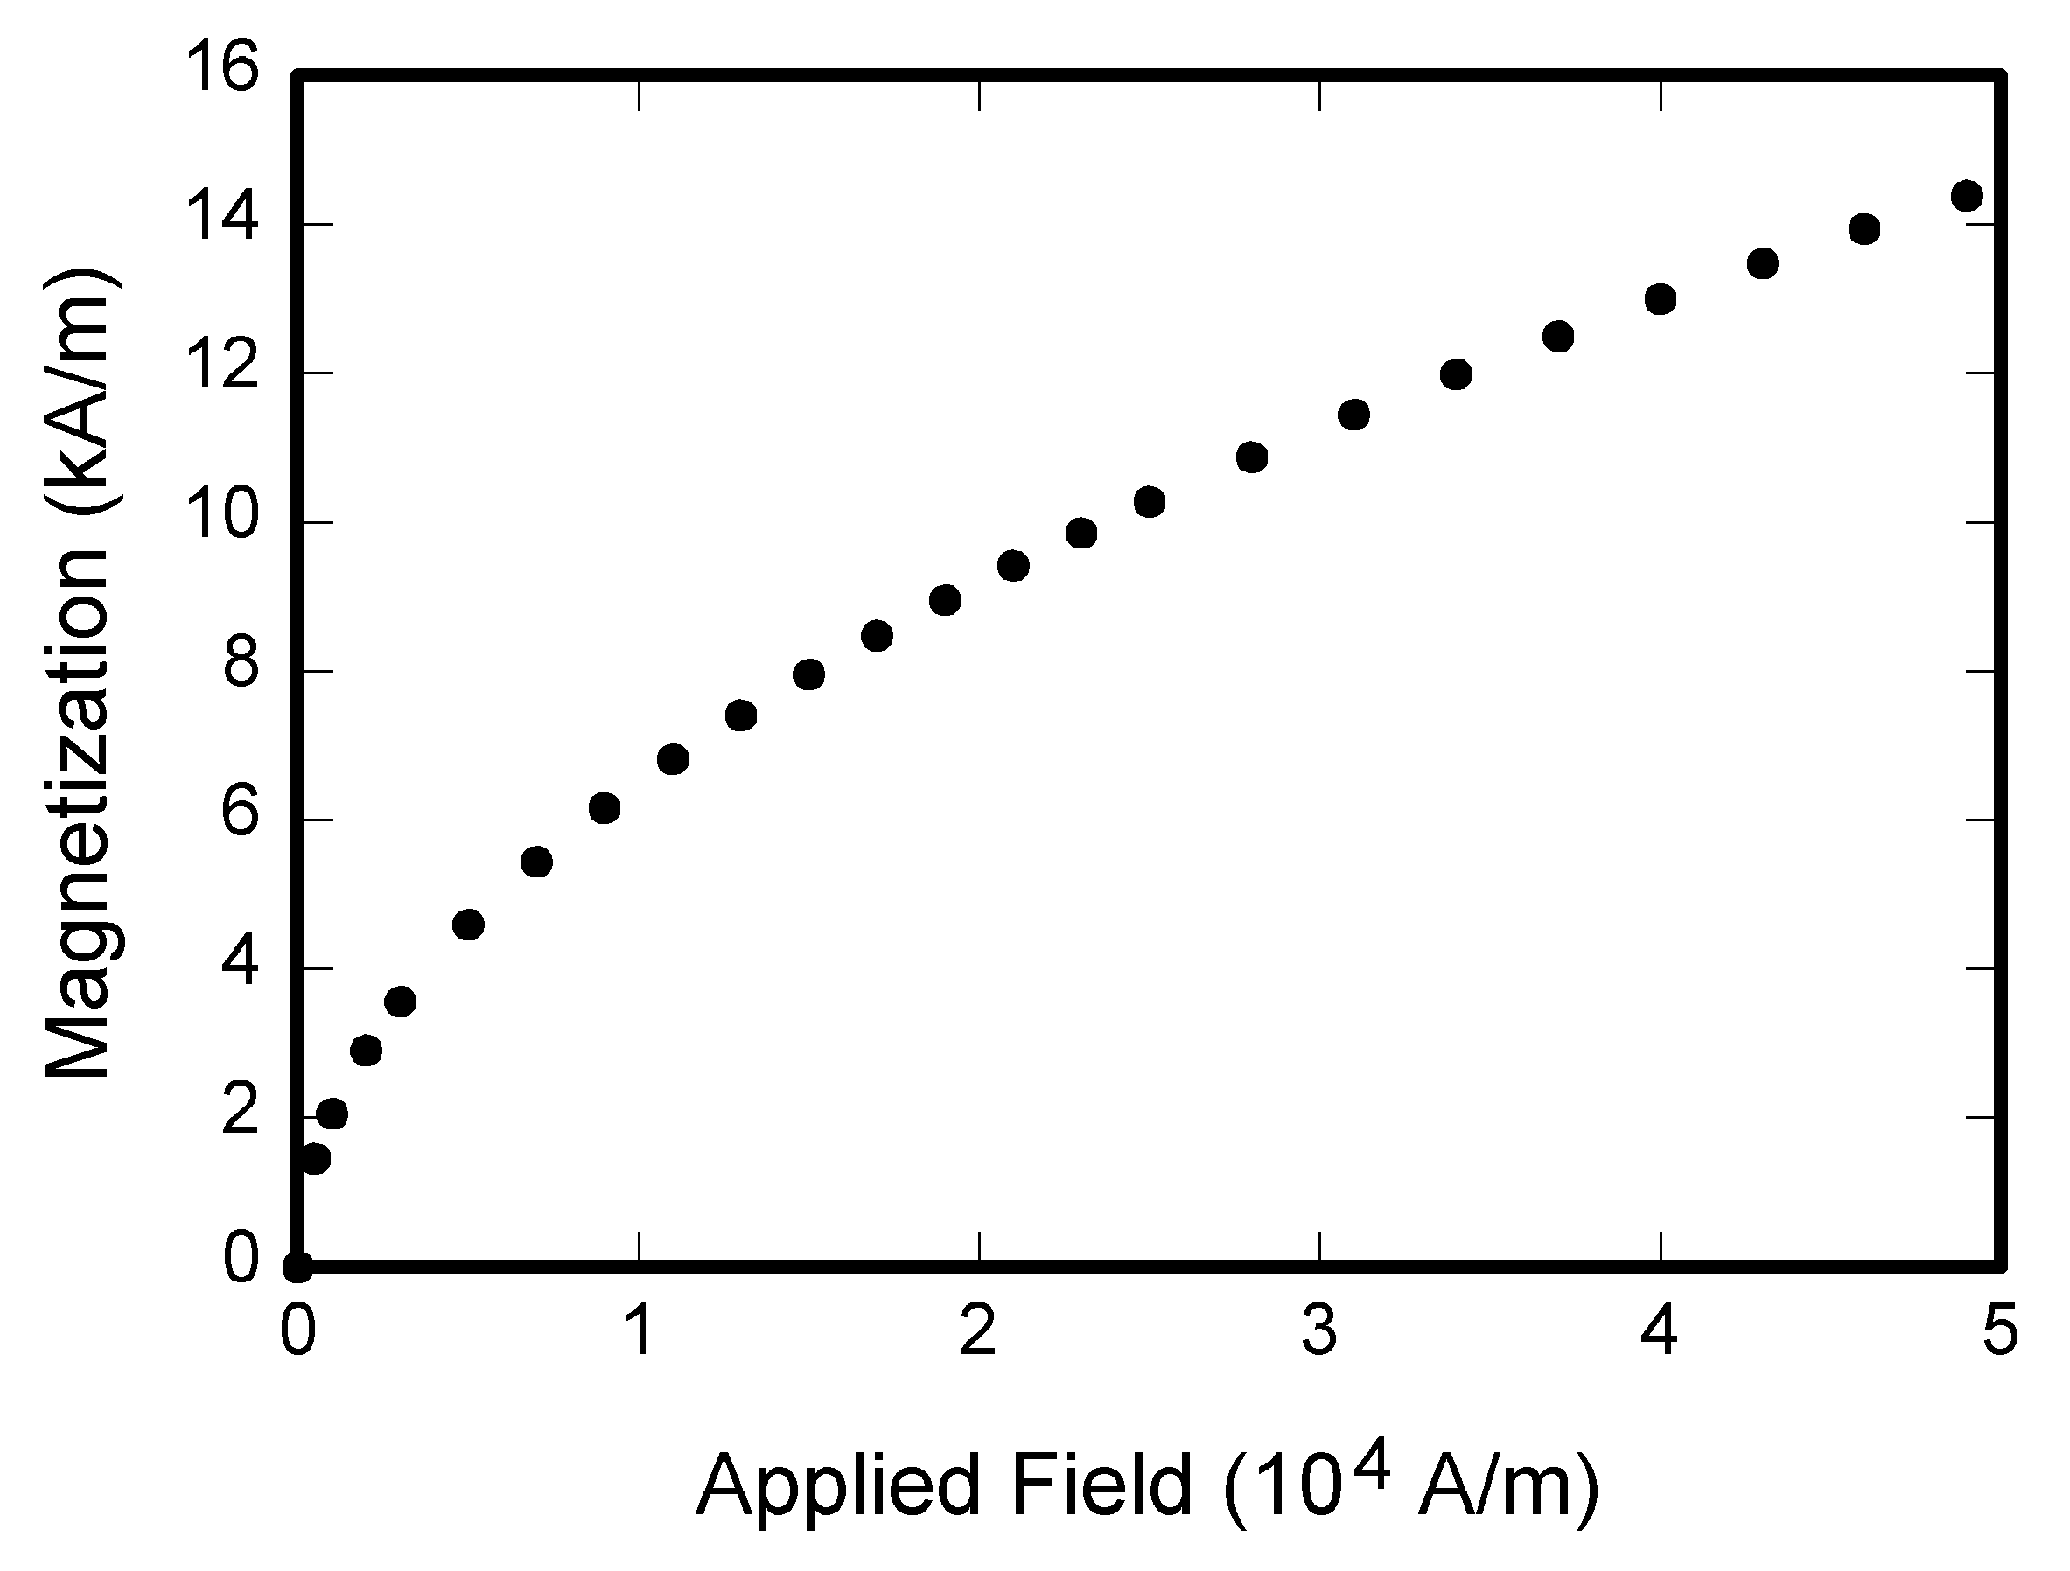
\includegraphics{fig1.png}}
\caption{Example of a figure caption.}
\label{fig}
\end{figure}


\cite{bishop2006pattern}

\bibliographystyle{unsrt}
\bibliography{references}






\end{document}
